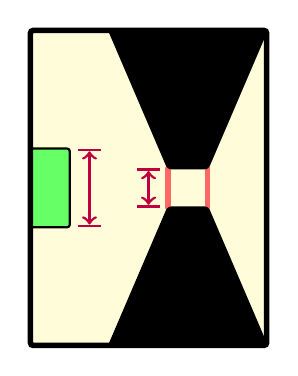
\begin{tikzpicture}[thick,scale=.5, every node/.style={scale=1}]

\begin{scope}

\clip (-1,0) -- (5,0) -- (5,8) -- (-1,8) -- cycle;

\draw [line width=0,fill=yellow!15!white] (-1,0) -- (5,0) -- (5,8) -- (-1,8) -- cycle;

\draw [red!60!white,line width=2,line cap=round] (2.5,3.5) -- (2.5,4.5);
\draw [red!60!white,line width=2,line cap=round] (3.5,3.5) -- (3.5,4.5);

\draw [fill=black,rounded corners=1] (1,0) -- (2.5,3.5) -- (3.5,3.5) -- (5,0) -- cycle;
\draw [fill=black,rounded corners=1] (1,8) -- (2.5,4.5) -- (3.5,4.5) -- (5,8) -- cycle;

\draw [fill=green!60!white,rounded corners=1] (-3,3) -- (-3,5) -- (0,5) -- (0,3) -- cycle;

\draw [arrows=|<->|,purple,line width=1pt,line cap=round] (0.5,5) -- (0.5,3);
\draw [arrows=|<->|,purple,line width=1pt,line cap=round] (2,4.5) -- (2,3.5);

\end{scope}

\draw [line width=2,rounded corners=1] (-1,0) -- (5,0) -- (5,8) -- (-1,8) -- cycle;

\end{tikzpicture}